\section{Data heterogeneity}
\label{sec:application}	

\begin{figure}[t]
	\centering
	\begin{minipage}{0.48\linewidth}
		\centering
   		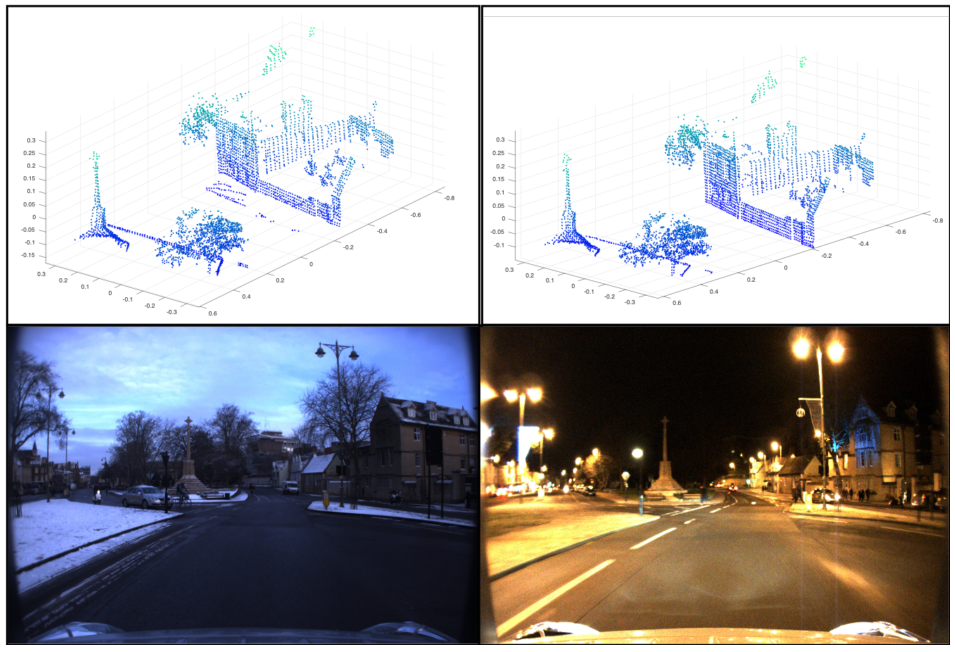
\includegraphics[width=\linewidth]{data_hetero/pointnetvlad.png}
	   		
   		\noindent\rule{\linewidth}{0.4pt}
   		   		
   		\subfigure[][Geometric information]{\label{fig:3d_info}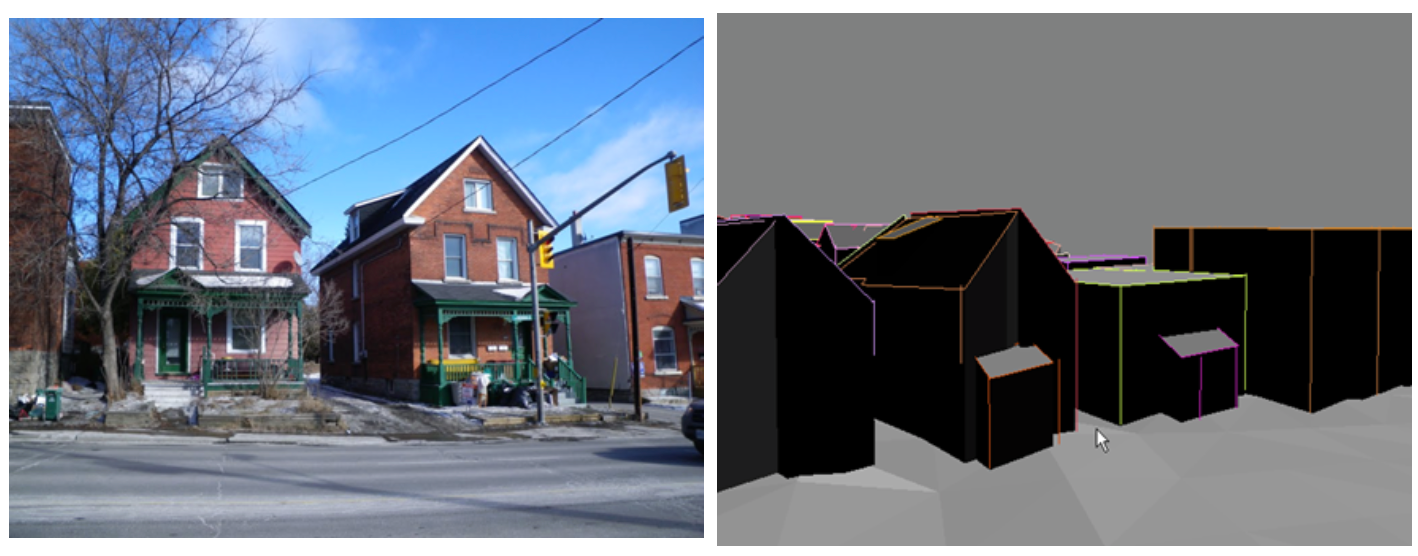
\includegraphics[width=\linewidth]{data_hetero/image_to_DEM.png}}
	\end{minipage}
	\begin{minipage}{0.48\linewidth}
		\centering
   		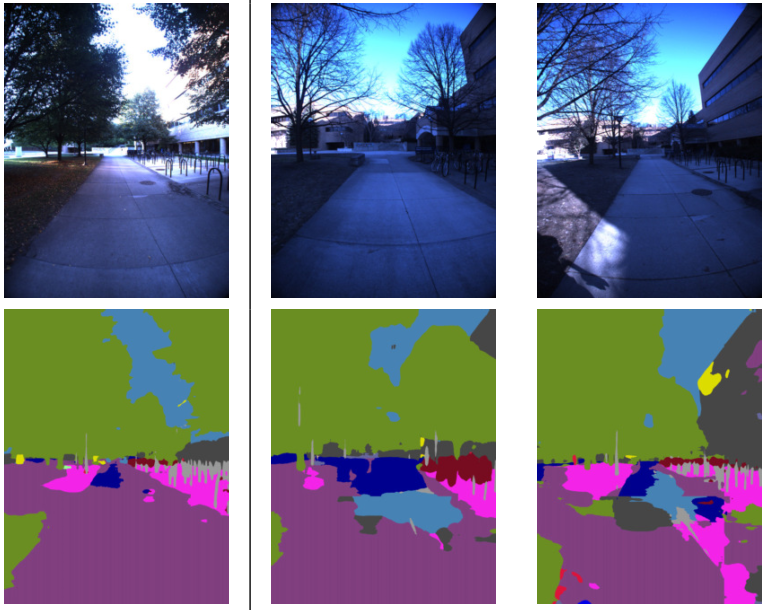
\includegraphics[width=0.95\linewidth]{data_hetero/semantic_vbl.png}
   		
		\noindent\rule{\linewidth}{0.4pt}		
		
   		\subfigure[][Semantic information]{\label{fig:seg_ifo}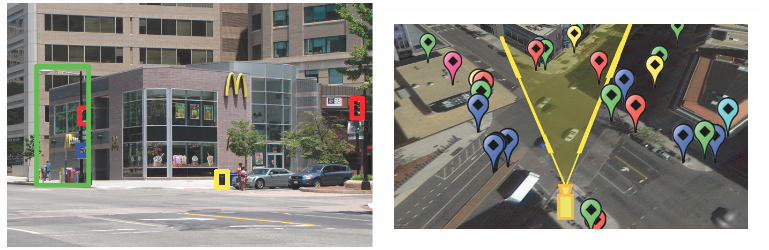
\includegraphics[width=\linewidth]{data_hetero/semantic.png}}
	\end{minipage}
	\caption[Illustration of the data heterogeneity in \ac{vbl}]{\textbf{Illustration of the data heterogeneity in \ac{vbl}:} \ref{fig:3d_info}~From top to bottom: PointNetVLAD~\citep{Uy2018} used to match point cloud for \acs{vbl} and localization system built upon a DEM~\citep{Matei2013}. \ref{fig:seg_ifo}~From top to bottom: data segmentation to help queries (right) to database (left) visual association ~\citep{Schonberger2017a} and localization system with semantic information gathered from OpenStreetMap annotation {Ardeshir2014}. \label{fig:data_div}}
\end{figure}

	Originally, pure-images were the dedicated data to \ac{vbl} systems~\citep{Robertson2004}. Still, conventional images for the task of localization have limitations, as mentioned in the previous section (see Section~\ref{sec:changing_environment}). The use of other type of data, such as geometric and semantic information, can circumvent these limitations.

	\subsection{Geometric information}
		\label{subsec:geometric_info}
		The growing accessibility of geometric data promotes the development of systems based on depth information~\citep{Paparoditis2012}. When available, depth information can directly improve the result of \ac{vbl} methods in term of robustness against visual changes and precision. We divide geometric information used in \ac{vbl} on four main categories:
		\begin{itemize}
			\item \textbf{Weak Geometry:} basic primitives like plans or simplified geometric model,
			\item \textbf{Point Cloud:} unordered set of 3D points, triangulated from images or acquired from lidar,
			\item \textbf{Depth Camera:} locally dense geometry obtained by active sensors,
			\item \textbf{3D Model:} full geometric model covering the area of localization, hand-crafted or generated from other sources.
		\end{itemize}
        
		\paragraph{Weak Geometry.}
			\label{subsubsec:weak_geometry}			
			In \citep{Torii2015,Chen2011}, authors introduce weak geometric clues that describe principal 3D planes present in the scene. This information is then used to modify existing images in the database: for rectification purpose~\citep{Chen2011} or to generate more images in order to cover a larger area~\citep{Torii2015}. \citet{Cham2010} use a 2D buildings outline map for \ac{vbl}. From a given image, authors extract buildings corner and match them according to the map. Along the same line, \ac{vbl} method from~\citep{Arth2015,Armagan2017a,Armagan2017b,Armagan2017} relies on a 2.5D map of Gratz (schematic buildings outlines boxes from OpenStreetMap\footnote{https://www.openstreetmap.org}). 2D map is also used as geo-reference in the work from~\citep{Brubaker2013} (extended version in~\citep{Brubaker2016}) where authors produce, thanks to a stereo-camera, a path of a vehicle that is afterwards matched against the map. The matching process is embedded in a probabilistic framework to handle large environment. \citet{Baatz2012} introduce the use of a \ac{dem} to perform localization in mountainous terrain~\citep{Ramalingam2010,Tzeng2013,Chen2015}. \citet{Bansal2014} extend this idea in urban localization to perform purely geometric \ac{vbl} with images as query input and \ac{dem} of a city as database. These purely geometric descriptions, also used in~\citep{Matei2013,Christie2016,Ramalingam2010,Ramalingam2011} (see figure~\ref{fig:3d_info}), permit localization independently of the illumination conditions.

		\paragraph{Point Cloud.}
        \label{subsubsec:3d_geometry}
			Previous section~\ref{subsubsec:sfm_methods} emphasizes the growing importance of colourized point clouds obtained by \ac{sfm} in \ac{vbl}~\citep{Irschara2009,Li2010,Sattler2011,Sattler2012,Sattler2015,Middelberg2014,Lynen2015,Lu2015,Svarm2014,Zeisl2015,Svarm2016,Sattler2016a,Feng2016a}. The addition of geometric relation by \ac{sfm} improves retrieval performances~\citep{Sattler2012a} and permits precise pose estimation of the query, on the contrary of methods based on simple images collections.
			
			In addition to the structured-based methods, some works focus on the localization of non-photogrammetric point cloud (\ie not create from images with \ac{sfm} algorithms), for instance acquired by laser scans~\citep{Elbaz2017,Uy2018,Schonberger2017a,Zeng2016,Yew2018,Deng2018}. From these methods, we can distinguish between global~\citep{Uy2018,Schonberger2017a} and local~\citep{Elbaz2017,Zeng2016,Yew2018,Deng2018} point cloud description. Fluctuation in point density is handle trough 3D automatic completion with an autoencoder in~\citep{Schonberger2017a} and by projection the 3D points in 2D in~\citep{Elbaz2017}. In order to be more robust to view point changes, methods in~\citep{Yew2018,Deng2018} process points in an unordered manner. By considering only the geometric structure of the scene, such methods are prone to handle radiometric changes present in long-term localization scenario, as illustrate in~\citep{Schonberger2017a,Uy2018} (see top of figure~\ref{fig:3d_info}).

		\paragraph{Depth Camera.}
			\Ac{sfm} reconstruction is a costly operation and laser sensor can be expensive and cumbersome for embedded \ac{vbl} application. Depth cameras permit a direct and cheap perception of the 3D geometry of the scene (\textit{e.g.} stereo camera, IR pattern projective camera, \ac{tof} camera, etc.). Raw data from those depth sensor are often used to add supplementary information channel to the \ac{vbl} system. Works from~\citep{Ni2009,McManus2014,Wan2014} use disparity map from stereo camera. Several authors~\citep{Shotton2013,Guzman-rivera2014,Glocker2015} used active depth camera that project infra-red pattern to train regression forest for localization. Similar technology is used in~\citep{Li2016a} to perform \ac{vbl} in complete obscurity. In the work of~\citep{Fernandez-Moral2013}, authors consider planar surfaces extracted from an RGB-D live stream as sustainable information for localization. The plane are organized within global graph where the pose of the camera can be retrieved quickly through sub-graph to global-graph matching.  However, depth camera are not well suited for outdoor uses, reducing the range of applications to indoor scene only.

		\paragraph{3D Model.}
			Consistent 3D models (\ie watertight 3D reconstruction) are also used to perform \ac{vbl} task.  For indoor localization, works from \citep{Shotton2013,Pascoe2015,Taira2018,Taira2019} use textured model reconstructed from RGB-D sensor~\citep{Shotton2013} or hand-crafted with dedicated software~\citep{Pascoe2015}. \citet{Salas-Moreno2013} introduce \ac{cad} models to describe objects in an indoor environment and recover the pose of a depth camera when the pose tracking is lost. City-scale models are used by \citep{Aubry2014,Poglitsch2015,Pascoe2015a,Pascoe2015b,Caselitz2016} to perform outdoor \ac{vbl}. 

	\subsection{Semantic information}
		\label{subsec:semantic_info}
		Robustness and precision brought by geometric information has a significant cost in term on data acquisition, processing power and storage needs. Nevertheless, there is a good alternative and discriminant data representation: the semantic information. In addition to being generic regarding the original ``raw'' scene representation, semantic abstraction permits a discriminative and robust description of the scene. Semantic information used in \ac{vbl} are classified between two classes: segmentation and categorization. Segmentation involves local methods that recognize within a data sub-parts with a semantic meaning (\eg object detection in an image). On the other hand, categorization can be seen as global descriptors that associated semantic labels to a given data (\eg scenes interpretation~\citep{Deng2009}).
		
		\paragraph{Segmentation.}
			 In~\citep{Ardeshir2014,Castaldo2015,Christie2016,Weinzaepfel2019}, authors use object to object semantic correspondences to directly recover the pose of the query (illustration on figure~\ref{fig:seg_ifo}). \citet{Weinzaepfel2019} create an object-of-interest database for localization. They demonstrate the robustness of their method to illumination changing on a synthetic museum dataset, where the object-of-interest are the paintings in a gallery. In~\citep{Lu2015}, semantic segmentation is used to narrow the search scope by aggregating information about the detected objects in a room.

 			 In a different manner, \citet{Arth2015} present concrete application of semantic segmentation for localization by extracting building primitives to correct pose hypothesis (the image is segmented with a \ac{svm} classifier). In following works~\citep{Armagan2017a,Armagan2017b,Armagan2017}, the image localization is performed by segmenting principal semantic components (facades, normal to facades, corners, etc.) of a building and by optimizing the query pose based on this segmentation and a map. They use \ac{cnn} trained in a weakly supervised manner to densely extract the architectural elements of buildings. On the other hand, several methods rely on annotated map~\citep{Atanasov2016,Wang2015} or \ac{gis}~\citep{Ardeshir2014,Castaldo2015,Qu2015} to guide the localization.
 			
			 Works described in~\citep{Arandjelovic2014a,Mousavian2015} consider the re-weighting of extracted local features in image according to the semantic class of the pixel obtained by image segmentation. Using this information, authors reduce the influence of local features that are not semantically robust for \ac{vbl}, like vegetation or cars. Thanks to progress in \ac{dl}, specially in image semantic segmentation, new methods based on \ac{cnn} have been successfully used to enforce coherence of local matching between images for localization~\citep{Shi2019,Toft2018,Taira2019}.
			 
			 \citet{Schonberger2017a} used latent representation computed by an autoencoder as global features for localization. They show that incorporating semantic segmentation information into the model representation improves significantly the localization performances of their descriptor. Similar conclusion are drawn in these following works~\citep{Seymour2018,Radwan2018} In~\citep{Garg2018,Garg2018a}, authors explicitly model the semantic classes of feature associated to a given region for localization of images with extreme view-point changes.
	    	
		\paragraph{Categorization.}
			Scene categorization~\citep{Wu2009} is a different manner to exploit semantic clues for \ac{vbl}. High level semantic features have been popularized with the augmentation of labelled data and the accessibility of high computation power devices (GPU, Cloud Computing). ImageNet challenge introduced in 2009 by~\citep{Deng2009} permits the emergence of fast and robust classification methods, like the one described in~\citep{Krizhevsky2012}. Image classification produces a sub-sample of semantically identical images associated to a class. In \ac{vbl}, classification can be used to decimate the database in order to proceed in a subsequent step to a more precise pose search. This method is successfully applied in~\citep{Sunderhauf2015}, where the used \ac{cnn} has a dual-purpose: narrowing the search scope by semantic labelling and producing a global descriptor by weight aggregation. In~\citep{torralba2003context,Ni2009}, classical learning methods like Gaussian Mixture Models (GMM) or epitome are employed for associating images to a finite number of possible locations. Recent work from~\citep{Garg2017} use semantic categorization in order to establish transition probabilities from a given type of environment to another one. Authors embed this framework in the SeqSLAM algorithm, improving the global system accuracy. Finally, works presented in~\citep{Weyand2016,Seo2018} consider the problem of world-wide localization as a classification task. A \ac{cnn} is trained to predict, from an raw image, its most probable location among a fixed number of Earth places.

	\subsection{Other modalities}
	\label{subsec:other_modalities}
	
	Geometric and semantic are the principals modalities used in common with radiometric information to improve \ac{vbl}. Yet, some works rely on thermal imaging~\citep{Lu2016}, infrared sensor~\citep{Bonardi2017} or polarimetric cameras~\citep{Rastgoo2018}. Thermal imaging makes possible the pose estimation of a camera in challenging low-light scenario~\citep{Lu2016}. On the other hand, sun light waves measurement from polarimetric cameras enables attitude estimation in unknown outdoor environment~\citep{Rastgoo2018}.
				
	\subsection{Cross-data localization}
	\label{subsec:cross_data}        
		We have presented so far three different kinds of information that can be used for \ac{vbl}: radiometric, geometric and semantic. These types of data are commonly used together to improve localization. In this part, we consider the scenario where all types of data are not available at query time, for instance if the database uses more complete representation of the environment than the query input. It is a common scenario because some data are more difficult to acquire or required specific sensors (\eg geometric information). In this case, methods have to deal with asymmetric representation of the environment in term of data type. We denote this problem cross-data \ac{vbl} and classify the methods founded in the literature in two categories: methods using a common description regardless of the type of data and methods projecting one type of data within another data representation space.
		
    	\paragraph{Common description.}
    		Features to Points (F2P) \ac{vbl} (see \S\ref{subsubsec:sfm_methods}) oppose 2D images to 3D point cloud. In fact, all the features are exclusively extracted from images. On the other hand, semantic abstraction permit cross-data comparison by considering semantic object extracted from various types of data: images to 2D building outline map~\citep{Cham2010}, images to map~\citep{Ardeshir2014,Qu2015,Castaldo2015,Brubaker2016}, RGB-D data to \ac{dem}~\citep{Christie2016}, etc. Referring to a similar physical entity, not necessary semantic, is also a manner to link information from various types of data. Images to DEM correspondences is performed in \citep{Bansal2014} based on a method relying on purely geometric clues extracted both in the image and the model. Recent work from \citep{Sizikova2016,Li2017} use joint descriptors to merge RGB and depth data into a single feature.
					
		\paragraph{Data projection.}
			Another widely used method for combining data of different types consists of projecting one of the engaged data into the representation space of the other. For instance, lot of methods consider the challenging problem of registering photographies upon 3D models~\citep{Baatz2012,Kendall2015,Arth2015,Pascoe2015,Pascoe2015a,Pascoe2015b}. Similarity comparison is performed thanks to synthetic images generated from the 3D models \citep{Russell2011,Mason2011,Aubry2014,Poglitsch2015,Taira2018,Taira2019}. Notice the synthesis of skyline profiles from DEM in the work of \citet{Baatz2012}. In~\citep{Irschara2009,Gee2012,Aubry2014,Torii2015}, special attention is paid to placement of the artificial cameras that generate virtual 2D views. 

			Generative model that create auxiliary modalities from images~\citep{Zamir2018} are promising tools for cross-data localization. \ac{cnn} that deduce relative geometry (normal direction) and semantic segmentation from raw images have been successfully used in~\citep{Taira2019} for indoor localization.

%	\begin{table}[t]
	\centering
	\caption[Data heterogeneity in \ac{vbl}]{\label{tab:data_types}\textbf{Data heterogeneity in \ac{vbl}.} Summary of the various types of data used in \ac{vbl}. First row indicates the type of data present in the database and the first column the type of the query confronted to this database. References in \textbf{bold} denote works using semantic interpretation of the data (see \S\ref{subsec:semantic_info}). $^{\dagger}$~Image-retrieval based methods that compare a input image to a set of images. Numerous references not displayed to readability reason. $^{\ddagger}$~Several works consider \ac{vbl} with as an input a set of images from the same scene rather than only one image input.}

	\renewcommand{\arraystretch}{1.1}
	\newcolumntype{M}[1]{>{\centering\arraybackslash}m{#1}}
	\footnotesize{
	\begin{tabular}{|m{0.13\textwidth} || M{0.18\textwidth} | M{0.18\textwidth} | M{0.18\textwidth} | M{0.18\textwidth} |}
          \hhline{-||----}
		\hfill \bf Database		& Images collection 				& Weak geometry					& SfM						& 3D model \\
          \bf Query 			& \S\ref{subsec:visual_info}			& \S\ref{subsubsec:weak_geometry}		& \S\ref{subsec:sfm_methods} 	& \S\ref{subsubsec:3d_geometry} \\
          \hhline{=::=:=:=:=:}
          Image				& Similarity search$^{\dagger}$ \textbf{\citep{Arandjelovic2014a,Garg2017,Mousavian2015,torralba2003context,Ni2009,Weyand2016}} 		& \citep{Baatz2012,Cham2010,Chen2011,Torii2015} \textbf{\citep{Atanasov2016,Ardeshir2014,Arth2015,Castaldo2015,Wang2015}} &  \citep{Arth2009,Donoser2014,Heisterklaus2014,Irschara2009,Feng2016a,Li2010,Li2012,Lu2015,Lynen2015,Middelberg2014,Sattler2011,Sattler2012,Sattler2015,Sattler2016a,Svarm2014,Zeisl2015}	& \citep{Aubry2014,Mason2011,Russell2011} \\
            \hhline{-||-|-|-|-|}
            Several images$^{\ddagger}$	& \citep{Weyand2016,Zamir2010}		& \citep{Brubaker2016} & \citep{Kroeger2014}								& \textbf{X} \\
            \hhline{-||-|-|-|-|}
            Image + Depth				& \textbf{X}						& \textbf{\citep{Christie2016}}						& \textbf{X}								& \citep{Cavallari,Gee2012,Glocker2013,Glocker2015,Guzman-rivera2014,Shotton2013,Valentin2015,Sizikova2016} \textbf{\citep{Fernandez-Moral2013,Salas-Moreno2013}}\\
            \hhline{-||-|-|-|-|}
            SfM				& \textbf{X}						& \textbf{X}						& \citep{Middelberg2014} \textbf{\citep{Lu2015}}				& \textbf{X} \\
            \hhline{-||-|-|-|-|}
	\end{tabular}
	}
\end{table}
	
To conclude this section, the different types of data used in \ac{vbl} methods are summarized in table~\ref{tab:data_types} (table in construction).

